\part{Latex}
    \section{Der Ursprung von \latex}
    Die Software \tex ist ein von Donald E. Knuth entwickeltes System um Texte jeglicher Art, aber vor allem wissenschaftliche Texte zu verfassen. Aufbauend auf der Basis-Software \tex entwickelt Leslie Lamport seit den 1980er Jahren eine Sammlung von \tex-Makros (genannt \latex). Diese Tex-Makros dienen hauptsächlich dazu, dass verfassen von Texten mit \tex zu vereinfachen. Die Grundidee von \latex ist das Vernachlässigen von Design-Entscheidungen während des Verfassens eines Textes. Ein Autor soll sich dementsprechend hauptsächlich auf die Inhalte des Textes konzentrieren können. Durch die Nutzung von \latex-Befehlen, werden die Inhalte anschließend durch den Kompiliervorgang formatiert. Mit \latex lassen sich Dokumente wie Artikel, technische Berichte, Bücher und Präsentationen anfertigen.

    \section{WYSIWYG}
    WYSIWYG ist das Akronym für What You See Is What You Get, dieses Prinzip beschreibt ein Verhalten von Textverarbeitungsprogrammen, in denen man schon während des Verfassens die finale Formatierung und das Aussehen des Textes zu sehen bekommt. Das bekannteste Beispiel für eine Software, welche nach diesem Prinzip funktioniert ist das Textverarbeitungsprogramm Microsoft Word.

    \tex hingegen verzichtet auf diesen Ansatz. Genau wie bei der Auszeichnungssprache (markup language) HTML wird die Formatierung, Gliederung und das Aussehen des Produkts durch eine eigene Syntax abgebildet und ist mit dem Inhalt vermischt. Um das fertige Produkt, das Dokument zu erstellen, ist ein Kompiliervorgang nötig. Dieses Prinzip wird auch als WYSIWYAF (What You See Is What You Asked For) bezeichnet.

    \section{Haupteinsatzgebiete für \tex}
    Besonders im naturwissenschaftlichen Bereich bietet sich die Auszeichnungssprache \tex an, da \tex eine komfortable Möglichkeit bietet Formeln oder Programmcode darzustellen. Ebenso lassen sich Abstände genau definieren (in Millimeter, Zentimeter usw.), was ein häufig wichtiges Kriterium für Wissenschaftliche Arbeiten darstellt. \tex bietet sich vor allem für Bachelorarbeiten, Masterarbeiten, Dissertationen und andere technische Arbeiten welche z.B. mathematische Inhalte enthalten an.

    Weitere komfortable und professionelle Möglichkeiten bietet \tex unter Anderem zum erstellen von Inhaltsverzeichnisses, Abbildungsverzeichnissen, Tabellenverzeichnissen, Literaturverzeichnissen und Glossaren.

\part{Atom}
    \section{Atom der hackable Text Editor}
    Atom ist ein vom Online-Dienst GitHub seit 2014 verfügbarer Text-Editor. Er ist frei verfügbar, open-source (MIT License) und plattformunabhängig. Entwickelt wurde der Text-Editor mit CoffeeScript, JavaScript, Less und HTML. Der Entwickler GitHub wirbt mit dem Slogan "`A hackable text editor for the 21st Century"'. Damit wird sich vor allem auf die Anpassbarkeit des Aussehens und das Verhaltens des Editor bezogen.

    Ebenso wie der Text-Editor selbst, sind auch die in Atom verfügbaren Packages (Plugins) in CoffeeScript bzw. JavaScript programmiert. Die Packages erweitern den Editor in seiner Funktionalität und werden sowohl von GitHub selber, so wie auch durch die Community erstellt und gepflegt.

    \section{Vergleichbare Editoren}
    Zur Einordnung des Atom Editors sollen an dieser Stelle einige Alternativen genannt werden. Neben Atom gibt es einige Editoren mit ähnlichen Konzepten. Der proprietäre, häufig als Vorlage zu Atom genannte Edtior Sublime Text von Jon Skinner. Der für Webdesign optimierte open source Editor Brackets von Adobe System und der von Microsoft angebotene open source Code Editor Visual Studio Code. Jeder dieser hat eine ähnliche Erscheinung, unter anderem eine Konsole oder Command Palette, eine Baumansicht zur Datei und Verzeichnis Übersicht und verschiedene Designs. Ebenso werden für all diese Editoren Plugins bzw. Packages, also im allgemeinen Erweiterungen angeboten. Eine besondere Gemeinsamkeit habe Atom und der Visual Code Editor in ihrer Grundlage, beide Editoren sind mit dem von GitHub entwickelten Framework "`Electron"' entwickelt worden. "`Electron"' erlaubt es Desktop Applikationen mit dem Node.js Framework zu erstellen.

\part{Atom Packages}
\section{Aufbau eines Atom Packages}
    \begin{figure}[H]
        \begin{minipage}{0.6\textwidth}
            Wird eine neues Package im Atom Editor angeleget, wird die in Abbildung \textit{Atom Package Struktur} gezeigte Verzeichnis- und Dateistruktur angelegt. Ausgenommen der Konfigurationsdateien \texttt{.eslintrrc.js, .gitattributes, .gitignore, .tern-project}, welche nachträglich hinzugefügt worden sind und die Entwicklung des Packages erleichtern. Das Grundgerüst und die Grundvoraussetzungen um eine neues Package mit Atom anzulegen sind also schon durch den Editor selbst gegeben.
        \end{minipage}
        \begin{minipage}{0.4\textwidth}
            \centering
            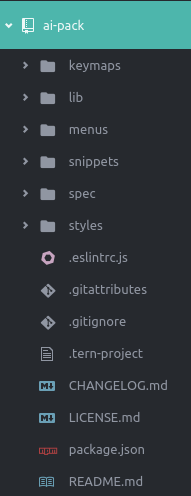
\includegraphics[scale=0.5]{img/package_structure.png}
            \caption{Atom Package Struktur}
        \end{minipage}
    \end{figure}

    \begin{minipage}{\textwidth}
        Die für das RookieTeX Package wichtigsten Verzeichnisse sind \texttt{lib} und \texttt{snippets}. Im Verzeichnis \texttt{lib}    befindet sich die Logik des Packages bestehend aus den Dateien: \\[5mm]
        \begin{tabular}{ | c | p{0.7\textwidth} | }
            \hline
            \textbf{Dateiname} & \textbf{Zweck} \\
            \hline
            \texttt{ai-pack-view.coffee} & Einstiegspunkt des Packages \\
            \hline
            \texttt{ai-pack.js} & Deklaration von Command Palette Befehlen und Package Einstellungen \\
            \hline
            \texttt{converter.js} & Funktionen zur Konvertierung von Text in \tex \\
            \hline
            \texttt{generator.js} & Funktionen zur Generierung eines \tex-Projekts \\
            \hline
            \texttt{templates.js} & Funktionen zur Generierung von \tex Elementen \\
            \hline
            \texttt{utils.js} & Hilfsfunktionen \\
            \hline
        \end{tabular}
    \end{minipage} \\[5mm]
    Im Verzeichnis \texttt{snippets} befindet sich ausschließlich die Datei \texttt{latex-snippets.cson}. Diese Datei im CoffeeScript Object Notation Format beinhaltet jegliche Snippets des Package, im Fall von RookieTeX also \latex Snippets. Die Snippets haben folgende Form:
    \\[5mm]
    \insertcode{src/example_snippet.cson}{\latex Snippet Beispiel (\latex Tabelle)}

    Zeile 1 benennt das Snippet. Zeile 2 gibt das auslösende Prefix an, welches genutzt wird um das Snippet zu verwenden und Zeile 3 bis 8 spiegeln den bei Verwendung eingefügten Inhalt des Snippets wieder. Ein wichtiger Aspekt sind die in Zeile 5 und 6 zu sehenden Tab-Stops, welche nach dem Einfügen des Snippets-Body's dafür sorgen, dass der User mithilfe der Tab-Taste die Inhalte des \tex-Befehls füllen kann.
    \\
    Des Weiteren wird in dieser Datei festgelegt welche Art von Dateien die enthaltenen Snippets auslösen/triggern können oder auch welche \textit{Scopes} die Snippets verwenden können. Im konkreten Fall von RookieTeX ist die Definition der unterstützten Formate/Scopes folgende: \texttt{'.text.plain, .text.latex':}. Es ist also bei der Bearbeitung von Plain Text oder \latex-Text möglich enthaltenen Snippets zu nutzen.
    \\
    Im Hauptverzeichnis befindet sich des Weiteren die Datei \texttt{package.json}, diese Datei stellt eine Art globale Konfigurationsdatei für das Package dar. Hier werden Dinge wie der Name, Beschreibung, Version, Command Palette Kommandos und Abhängigkeiten zu anderen JavaScript Bibliotheken festgelegt.
    \insertcode{src/example_package.json}{Ausschnitt der package.json Datei des RookieTeX Packages}

    \section{Gegenüberstellung von JavaScript und CoffeeScript}
        CoffeeScript ist ein open-source Projekt (MIT License). In CoffeeScript geschriebener Code wird zu JavaScript transcompiliert, das heißt jedes CofeeScript-Konstrukt hat ein Equivalent in JavaScript, welches zur Laufzeit übersetzt wird. Das Hauptaugenmerk von CoffeeScript ist es eine neue Syntax zum schreiben von JavaScript Programmen anzubieten. CoffeeScript ist nicht das einzige Projekt mit diesem Zweck, auch beispielsweise TypeScript oder Dart bieten ähnliche Möglichkeiten. Der Vorteil dieser neuen Syntax ist eine kürzere, übersichtlichere, kompaktere Erscheinung und schnelleres schreiben des Codes, wobei zu beachten ist, dass die Lesbarkeit zum Teil eine subjektive Bewertung ist. Der Stil von CoffeeScript erinnert an Programmiersprachen wie Python und Ruby. Als problematisch stellt sich das Debugging von CoffeeScript Programmen dar, da der kompilierte Code trotz nutzen von CoffeeScript Syntax weiterhin in JavaScript Syntax vorliegt. Beginnt man also statt JavaScript direkt mit CoffeeScript, ist man auf sogenannte "`Source Maps"' angewiesen. Diese "`Source Maps"' zeigen dem Entwickler während dem Debugging für jedes JavaScript Konstrukt das dazu passende CoffeeScript Konstrukt an.
        \\
        Die Entscheidung RookieTeX in JavaScript, statt der von Atom vorgegebenen "`Sprache"' CoffeeScript zu entwickeln hatte mehrere Gründe. Zum einen gibt es eine ausreichende Menge qualitativer Werkzeuge um das Programmieren von JavaScript komfortabler zu machen (Autovervollständigung usw.). Des Weiteren ist JavaScript weiter verbreitet, also CoffeeScript, was den Vorteil hat, mehr Inhalte und Unterstützung für JavaScript im Internet zu finden. Die Community ist größer. Nicht zu Letzt scheint JavaScript subjektiv betrachtet eine größere Marktpräsenz vorzuweisen.

    \section{Nutzen und Einsatzgebiet von RookieTeX}
    Das Package RookieTeX dient dazu, Verfassern von \tex-Dokumenten die Erstellung von Dokumenten zu erleichtern. Vor allem neuen \latex Benutzern soll mithilfe des Atom Editor in Verbindung mit RookieTeX ein leichterer Einstieg in \latex angeboten werden. Zwar gibt es auch Zahlreiche andere \latex-Editoren auf dem Markt, viele davon sind allerdings mit sehr vielen Funktionen ausgestattet die für den Einstieg in \tex nicht förderlich sind, da sie den Benutzer überfordern. Um die Funktionsweise von \latex zu verstehen, ist es des Weiteren wichtig den unkompilierten \latex-Code selbst zu schreiben und auch lesen zu können. Editoren die den Ansatz verfolgen das Prinzip WYSIWYG mit \latex zu kombinieren, wiedersprechen dem eigentlichen Konzept von \latex.
    \\
    Der Atom Text-Editor soll in Verbindung mit dem Package folgende Funktionalitäten bieten.
    \\[5mm]
    \begin{itemize}
        \item Anlegen eines \tex-Projekts mit einer wartungsfreundlichen Verzeichnis- und Dateistruktur.
        \item Optionale Generierung von Glossar und Vorlage zum einfügen von Code durch Package Einstellungen.
        \item Sammlung von Snippets, die entweder im Editor direkt oder durch die Command Palette eingefügt werden können.
        \item Konvertierung/Formatierung von bereits vorhandenem Text.
    \end{itemize}

    \section{Funktionalitäten von RookieTeX}
        \subsection{Generierung eines \latex-Projekts}
            Bei der Generierung eines \latex-Projekts (\texttt{InitializeTexProject}) über die Command Palette wird eine Vorlage für ein \latex-Projekt im Dateisystem angelegt. Der Speicherort ist von der Einstellung des RookieTeX Packages abhängig, dort kann je nach Wunsch festgelegt werden, wo die benötigten Dateien und Verzeichnisse abgelegt werden.
            \begin{figure}[H]
                \centering
                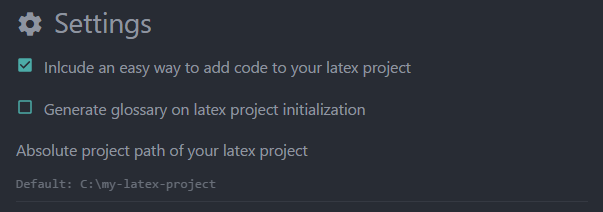
\includegraphics[width=\textwidth]{img/package_settings.png}
                \caption{RookieTeX Package Settings}
            \end{figure}
            Zusätzlich zum verwendeten Speicherort, kann entschieden werden, ob das Projekt für die Einbindung von Source Code vorbereitet werden soll und ob ein initiales Glossar mit erstellt wird.

        \subsection{Konvertierung von Plain Text Listen}
            Das RookieTeX Package bietet eine Konvertierung für geordnete und ungeordnete Listen, welche im Plain Text Format vorliegen an. Dazu wird eine Liste mit Spiegelstrichen oder nummerierter Aufzählung markiert und anschließend der Befehl \texttt{convertListToTex} aus der Command Palette aktiviert.
            \\[5mm]
            \begin{figure}[H]
                \centering
                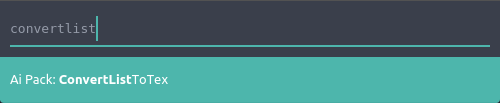
\includegraphics[width=0.7\textwidth]{img/convert_list_cp.png}
                \caption{Konvertierung einer Liste}
            \end{figure}

            \begin{figure}[H]

            Vor und nach der Konvertierung einer ungeordneten Liste: \\[5mm]
            \begin{minipage}[c]{0.45\textwidth}
                \begin{itemize}
                    \item[-] Bananen
                    \item[-] Äpfel
                    \item[-] Birnen
                \end{itemize}
            \end{minipage}
            \begin{minipage}[c]{0.1\textwidth}
                $\longrightarrow$
            \end{minipage}
            \begin{minipage}[c]{0.45\textwidth}
                \texttt{\noindent
                    \textbackslash{}begin\{itemize\} \\
                    \textbackslash{}item Bananen \\
                    \textbackslash{}item Äpfel \\
                    \textbackslash{}item Birnen \\
                    \textbackslash{}end\{itemize\}
                }
            \end{minipage}

            Vor und nach der Konvertierung einer geordneten Liste: \\[5mm]
            \begin{minipage}[c]{0.45\textwidth}
                \begin{enumerate}
                    \item Bananen
                    \item Äpfel
                    \item Birnen
                \end{enumerate}
            \end{minipage}
            \begin{minipage}[c]{0.1\textwidth}
                $\longrightarrow$
            \end{minipage}
            \begin{minipage}[c]{0.45\textwidth}
                \texttt{\noindent
                    \textbackslash{}begin\{enumerate\} \\
                    \textbackslash{}item Bananen \\
                    \textbackslash{}item Äpfel \\
                    \textbackslash{}item Birnen \\
                \textbackslash{}end\{enumerate\}
                }
            \end{minipage}
            \end{figure}

        \subsection{Formatierung/Konvertierung von Text}
            Das RookieTeX Package kann bereits vorhandenen ausgewählten Text fett, kursiv oder unterstrichen formatieren. Ist der Text markiert wird über die Command Palette die gewünschte Formatierung ausgewählt.
            \\[5mm]
            \begin{figure}[H]
                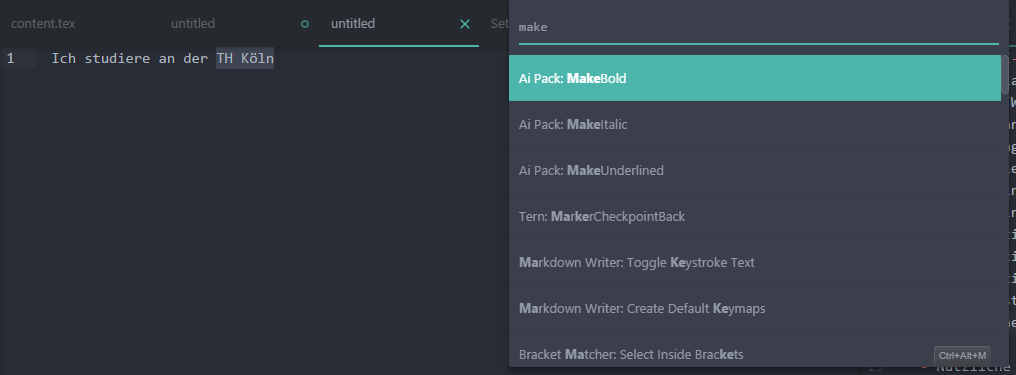
\includegraphics[width=\textwidth
                ]{img/make_bold_example.png}
                \caption{Konvertierung von markiertem Text}
            \end{figure}
            \begin{minipage}{\textwidth}
                \centering
                \begin{tabular}{ | l | l | }
                    \hline
                    \textbf{Plain Text} & \textbf{\latex Code} \\
                    \hline
                    fetter Text & \texttt{\textbackslash textbf\{fetter Text\}} \\
                    kursiver Text & \texttt{\textbackslash textit\{kursiver Text\}} \\
                    unterstrichener Text & \texttt{\textbackslash underline\{unterstrichener Text\}} \\
                    \hline
                \end{tabular}
            \end{minipage}

        \subsection{Nutzung von Snippets über die Command Palette}
            Neben der Aktivierung von Snippets mithilfe der Standardfunktionalität von Atom, also in dem spezifische Snippet Prefixe eingetippt werden, bietet RookieTeX die Möglichkeit Snippets über die Command Palette einzufügen. Die Command Palette dient dazu Befehle an den Editor abzusetzen. Durch bestimmte Befehle ermöglicht das Package nun \latex Snippets in den aktiven Editor-Tab an stelle des Cursors einzufügen. Der Zugriff auf Snippets über die Command Palette bietet den Vorteil, dass das Prefix des Snippets nicht bekannt sein muss, denn die Command Palette liefert ein Buchstaben-Matching innerhalb von Wörtern.
            \begin{figure}[H]
                \centering
                    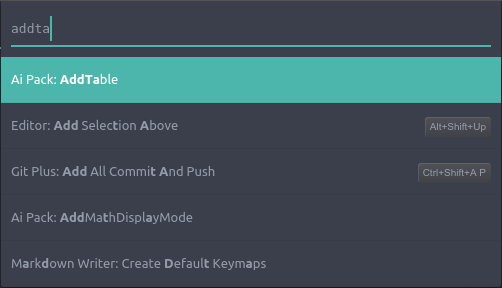
\includegraphics[scale=0.7]{img/snippets_via_cp.png}
                    \caption{Snippet via Command Palette einfügen}
            \end{figure}

\part{Aufbau eines \tex-Projekts}
    \section{Modulare Struktur eines \tex-Projekts}
    Um die Erstellung eines \tex-Projekts zu erleichtern, bietet es sich an eine modulare Struktur, also einen bestimmten Aufbau des Projekts zu nutzen. Es ist sinnvoll Dinge mit unterschiedlicher Semantik voneinander zu trennen. Zum Beispiel sollte sich ein Deckblatt oder ein Glossar nicht in der selben \texttt{.tex} Datei befinden wie der eigentliche Inhalt des im Projekt behandelten Themas. Des Weiteren sollten Projektübergreifende Einstellungen wie genutzte \latex-Packages oder Seitenabstände in einer \texttt{.sty} Datei zusammengefasst sein (Trennung von Design und Inhalt). Diese Vorgehensweise hat den Vorteil das besonders in umfangreichen Projekten die Übersicht gewährleistet wird. In den \texttt{.tex} Dateien die den eigentlichen Inhalt des zu erstellenden Dokuments beinhalten, kann sich so hauptsächlich auf das Schreiben von Text konzentriert werden. Design von Inhalten zu trennen ist, wie im Abschnitt "`Der Ursprung von \latex"' einer der Hauptvorteile \latex zu nutzen.

    \tex liefert verschiedene Möglichkeiten zum auslagern und modularisieren von \tex-Komponenten. Als Basisfunktion kann der \latex-Befehl \texttt{\\include} genannt werden, welcher dazu dient verschiedene \texttt{.tex} Dateien in einer Datei zusammenzuführen. Der \latex-Compiler sorgt dann automatisch dafür, dass alle \texttt{.tex} Dateien in der angegebenen Reihenfolge kompiliert werden. Diese Funktionalität arbeitet sowohl auf einer Verzeichnisebene, als auch Verzeichnis übergreifend.

\part{Implementierung}
    \section{Implementierung der Generierung eines \latex-Projekts}
        Um ein \latex-Projekt zu generieren, werden zunächst die Package-Settings eingelesen. Dies geschieht mit mitgelieferten Atom-API Funktionen. Auf Basis der ermittelten Angaben zur Einbindung von Glossar, Code Snippets und Projektpfad werden schließlich die zu erstellenden Dateien in Form von Strings gespeichert. Sind alle Dateiinhalte zwischengespeichert, werden die benötigten Verzeichnisse und Dateien mit Hilfe der Node.js Libraries \texttt{mkdirp} und \texttt{fs} erstellt. Dabei ist zu beachten, dass die Verzeichnisse synchron erstellt werden (Funktion: \texttt{mkdirp.sync(dir, opts)}). Das ist wichtig, da es sonst zur Laufzeit passieren kann, dass ein Unterverzeichnis parallel mit einem übergeordneten Verzeichnis erstellt wird, was einen Fehler und ein nicht korrekt erstelltes \latex-Projekt zur Folge hat.
        \\
        Damit die genutzten JavaScript Libraries dem Nutzer auch dann zur Verfügung stehen wenn diese nicht manuell installiert werden, sind diese in der Package-Konfigurationsdatei \texttt{package.json} eingebunden (Siehe Listing 2). In den \textit{dependencies} wird der Name der Library, gefolgt von der benötigten Version angegeben. Im Falle der Package-Installation werden dieses Libraries dann automatisch installiert.

    \section{Implementierung der Konvertierung von Plain Text Listen}
        Um bereits vorhandene Listen in \latex-Syntax zu konvertieren, wird zunächst der im Editor selektierte Text eingelesen und zwischengespeichert. Das einlesen selbst ist allein durch Atom-API Funktionen realisiert. Ist bei Funktionsaufruf kein Text selektiert, wird der Anwender mit Hilfe der JavaScript Funktion \texttt{alert} darüber informiert. Auch wenn der selektierte Text keine kompatible Liste enthält, wird der Benutzer in Form eines Popups informiert. Um die genannten Fälle erkennen zu können, werden zwei verschiedene Regex-Muster auf den eingelesenen Text angewendet. Hat nun kein Regex-Muster eine Übereinstimmung erkannt, kann keine \latex-Liste generiert werden. Für den Fall das eins der beiden Regex-Muster (entweder eine nummerierte Liste oder eine Liste mit Spiegelstrichen) Übereinstimmungen hat, wird der entsprechende \latex-Code zu einem String konkateniert und im Editor an stelle des zuvor selektierten Textes geschrieben.
        \\
        Die beiden Regex-Muster zu Erkennung der verschiedenen Listen sind folgendermaßen umgesetzt:
        \\[5mm]
        \begin{minipage}{\textwidth}
            \centering
            \begin{tabular}{ | c | c | }
              \hline
              \textbf{Listen-Typ} & \textbf{Regex-Muster} \\
              \hline
              Spiegelstrich-Liste & \texttt{'([-].+[\textbackslash n]){1,}', 'gm'} \\
              nummerierte Liste & \texttt{'([0-9].+[\textbackslash n]){1,}', 'gm'} \\
              \hline
            \end{tabular}
        \end{minipage}

    \section{Implementierung der Formatierung von Text}
        Ähnlich wie Konvertierung von Plain Text Listen zu \latex-Listen funktioniert auch das formatieren von ausgewählten Textabschnitten. Mit Hilfe von Atom-API Funktionen wird der markierte Text im Editor eingelesen und bearbeitet. Zur einfachen Formatierung sind in Gegensatz zur Listenkonvertierung jedoch keine Regex-Abgleichungen nötig. Um den Text ins \latex-Format zu überführen wird er mit der JavaScript Funktion \texttt{slice} bearbeitet, welche den markierten Text in die geschweiften Klammern des \latex-Befehls einfügt. Der zuvor selektierte Text wird anschließend durch den neu markierten Text ersetzt.

    \newpage
    \section{Implementierung der Nutzung von Snippets über die Command Palette}
        Erkennt der Atom Editor im eingegebene Text ein Snippet wird dieses in Form einer Auswahlvorschau angezeigt.
        \begin{figure}[H]
            \centering
            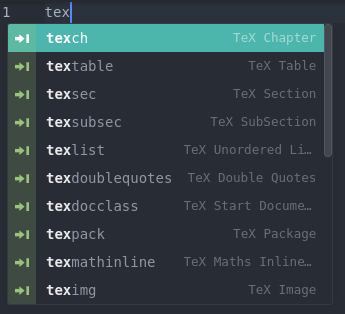
\includegraphics[scale=0.5]{img/snippet_preview.png}
            \caption{Snippet Auswahlvorschau}
        \end{figure}
        Im Normalfall wird das gewünschte Snippet dann direkt via Tab-Taste aktiviert oder erst per Pfeiltaste oder Maus ausgewählt und anschließend mit Enter bestätigt.
        \\
        Um Snippets über die Command Palette einfügen zu können, wurde das Einfügen von Snippets aufgrund nicht vorhandener API Funktionen, welche das aktivieren eins Snippets ermöglichen nach einem ähnlichen Prinzip implementiert. Wird ein Snippet in der Command Palette gesucht und ausgewählt, fügt die Funktion \texttt{insertText} der Klasse \texttt{Editor} das zugehörige Prefix für das gewünschte Snippet ein. Unmittelbar danach wird durch die Funktion \texttt{buildKeydownEvent} der Klasse KeymapManager der ein Betätigend der Tab-Taste simuliert, wodurch das gewünschte Snippet eingefügt wird.

    \section{Hindernisse und Probleme bei der Entwicklung von RookieTeX}
        In der Zeit der Entwicklung des Packages hat der Atom Editor vier Versions Updates bekommen, angefangen mit Version 1.4.0 und aktuell mit Version 1.5.3 (Stand: 18.02.2016). Parallel zu diesen Updates wird die Atom API (\href{https://www.atom.io/docs/api/}{Atom API Link}) gepflegt. Auffällig ist die sehr unterschiedliche Detailtiefe der API, während eine Klasse bis ins Detail beschrieben sind und auch Code Beispiele vorliegen, sind andere Klasse nur sehr knapp beschrieben und bieten keine Beispiele an. Teilweise wird somit die Implementierung eines Packages sehr erschwert, da häufig Community Foren oder Packages von anderen Entwickler herangezogen werden müssen, um Code Beispiele einzusehen.
        \\
        Wegen der teilweise schlechte bzw. nicht ausführlichen Dokumentationen von Klassen, bietet es sich also in gewissen Fällen an auf weiter verbreitete Node.js Klassen zurückzugreifen. Im Falle des RookieTeX Packages sind deshalb die externen Libraries \texttt{mkdirp} und \texttt{fs} zum Einsatz gekommen. Beispielsweise fehlt der Klasse \texttt{Directory} die Möglichkeit oder ggf. nur die Erklärung wie Verzeichnisse nicht asynchron sonder synchron erstellt werden können. Ein anderes Beispiel ist die für Einsteiger nicht ausreichende Beschreibung der Möglichkeit einen Tastendruck zu simulieren, welche in RookieTeX genutzt wird um Snippets via Command Palette auszuführen.

\part{Weiterführend}
    \section{Nützliche Atom Packages zum anfertigen von \latex-Dokumenten}
        \subsection{language-latex}
            Das \textit{language-latex} Package sorgt dafür das ein Syntax-Highlighting von \latex-Code im Editor stattfindet. \latex-Befehle werden also farblich hervorgehoben und sind leichter erkennbar. Im Atom Editor lässt sich die aktuelle Sprache dann über die standardmäßige Tastenkombination \texttt{Strg-Shift-L} die Sprache \latex auswählen. Dokumente mit der Dateiendung \texttt{.tex} werden außerdem automatisch erkannt.
        \subsection{latex}
            Das \textit{latex} Package erlaubt es dem Benutzer bei installierem \latex-Compiler, \texttt{.tex}-Dateien aus dem Editor heraus zu kompilieren.
        \subsection{linter-chktex}
            In Kombination mit dem \textit{linter} Package macht \textit{linter-chktex} eine Live-Überprüfung des vorhandenen \latex-Codes möglich. So können Fehler und unsaubere Schreibweise schon vor dem Compile-Vorgang entdeckt und beseitigt werden.
